\chapter{Lazart - Implémentation et expérimentations}
\label{chpt:lazart-implem}

\begin{tikzpicture}[remember picture,overlay]
\node[anchor=west,inner sep=0pt] at (current page text area.west|-0,3cm) {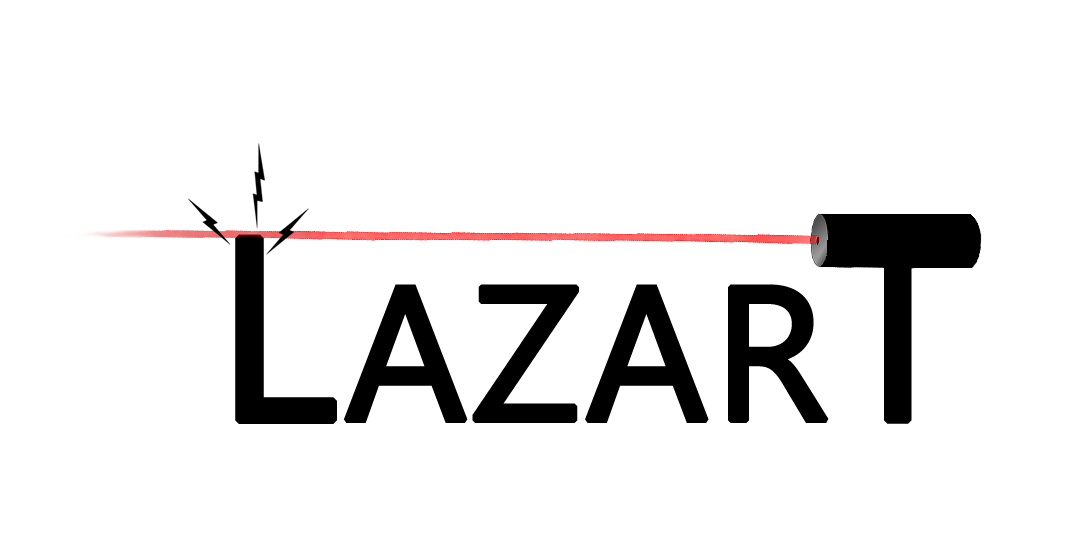
\includegraphics[height=3cm]{ch3-lazart/img/lazart-logo-red.png}};
\end{tikzpicture}

    Ce chapitre s'intéresse à l'implémentation de l'outil Lazart et discute des choix et compromis qui ont été faits.
    
    La section \ref{sec:lazart-impl-klee} décrit l'interaction entre Lazart et l'outil d'exécution concolique (KLEE).
    La section \ref{sec:lazart-impl-wolv} présente Wolverine (phase de mutation), son architecture et son fonctionnement.
    La section \ref{sec:lazart-impl-mfct} explique les choix d'implémentation concernant l'émulation des fautes.
    La section \ref{sec:lazart-impl-analysis} détaille l'implémentation et la complexité des analyses d'attaques de Lazart.
    Finalement, la section \ref{sec:lazart-conclusion} propose une synthèse des chapitres \ref{chpt:lazart} et \ref{chpt:lazart-implem}, ces deux chapitres sur l'outil Lazart et revient sur les contributions et les perspectives de l'outil.

    \setcounter{tocdepth}{2}
    \section*{Table des Matières}
    \localtableofcontents
    
    \section{Interaction avec KLEE}
    \label{sec:lazart-impl-klee}
    
        \begin{figure}[t]\centering
            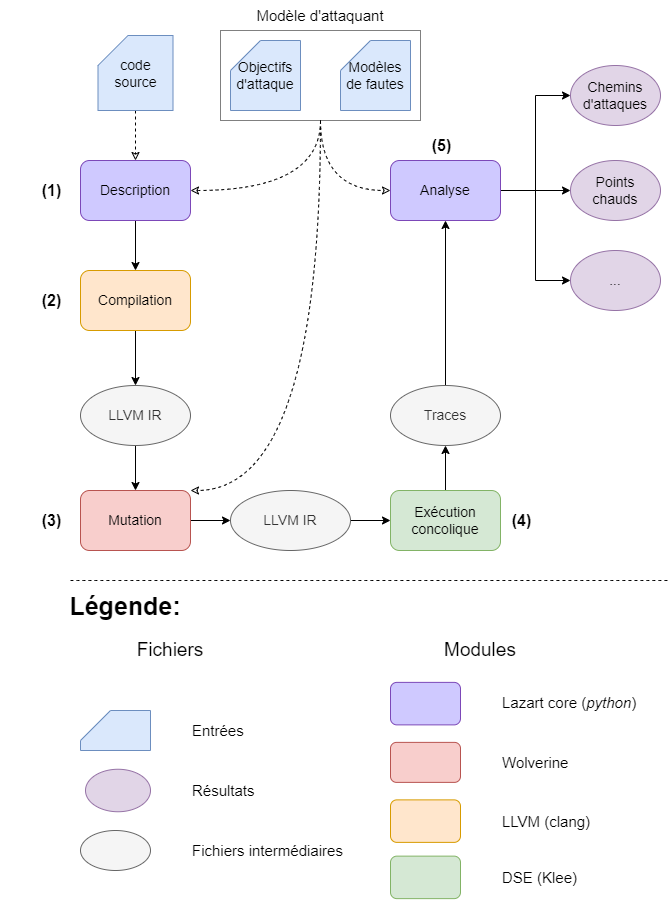
\includegraphics[scale=0.4]{ch3-lazart/img/lazart-workflow4_pack.drawio.png}
            \caption{Processus d'analyse avec Lazart (rappel)}  \label{fig:lazart-analysis-scheme-ch4}
        \end{figure}
    
        KLEE est appelé après la phase de mutation avec pour entrées le mutant \gls{llvm-ir} et des arguments paramétrables depuis l'\gls{api} Python (voir figure \ref{fig:lazart-analysis-scheme-ch4}). Une fois que l'exécution symbolique est terminée (ou bien la fin d'un timeout spécifié par l'utilisateur), la phase de lecture des traces permet de récupérer les résultats de KLEE et les convertir dans la représentation de Lazart.
        L'usage de KLEE nécessite de prendre quelques précautions:
        \begin{itemize}
            \item Retarder au maximum l'introduction de variables symboliques et de disjonction de chemins dues aux fautes.
            \item Couper les traces qui ne nous intéressent pas au plus tôt.
            \item Choisir un paramétrage de KLEE adapté aux besoins de l'analyse et évitant d'introduire une concrétisation non souhaitée.
        \end{itemize}
        
        Ces aspects sont à prendre en compte par l'utilisateur lors de l'instrumentation du programme et du paramétrage de Lazart, comme cela a été abordé dans le chapitre précédent (section \ref{lazart:metho}). 
        Ce sont aussi des problématiques qui ont été considérées lors de l'implémentation de l'outil.
        
        Les deux premiers points sont directement liés à la génération du mutant et à l'émulation des fautes, et seront abordés dans la section \ref{sec:lazart-impl-mfct}. Cette section se concentre sur la récupération des traces d'exécution à partir des cas de test et le paramétrage de KLEE.
        La section \ref{sec:lazart-impl-klee-replay} présente la méthode de rejeu utilisée par Lazart pour récupérer les chemins de KLEE.
        La section \ref{sec:lazart-impl-klee-read} s'intéresse aux optimisations concernant l'exploration des chemins de KLEE et la lecture des ktests par Lazart. 
        La section \ref{sec:userevent} décrit comment récupérer des propriétés sur les traces, par exemple pour vérifier plusieurs objectifs d'attaque en une seule analyse.
    
        \subsection{Rejeu des traces}
        \label{sec:lazart-impl-klee-replay}
 	
            Pour récupérer les données d'une trace à partir d'un cas de test fourni par KLEE (fichier \texttt{.ktest}), chaque évènement d'une trace (entrée dans un bloc de base, déclenchement d'une faute, etc) est affiché sur la sortie standard avec un format spécifique.
            Lazart utilise la fonctionnalité \textit{de rejeu} de KLEE (voir section \ref{sec:klee}) qui permet d'exécuter un ktest avec des entrées concrètes validant le prédicat de chemin de cette trace. La trace est ainsi reconstituée en analysant la sortie console de chaque rejeu de trace et transformée dans la représentation de Lazart.
            
\lstset{caption={Exemple de rejeu d'un ktest de KLEE},label=lst:replay-klee}
\begin{lstlisting}  
[TRACE] bb2
[TRACE] bb3
[FAULT] [DL] [2] [12] [0]
[TRACE] bb5
[USER] tmp = 12
...
\end{lstlisting} 

            Le listing \ref{lst:replay-klee} présente un exemple d'affichage console lors du rejeu d'une trace. 
            Chaque type d'évènement suit une syntaxe précise. Les lignes préfixées par \texttt{[TRACE]} correspondent à l'entrée dans un bloc de base et la ligne préfixée par \texttt{[FAULT]} correspond à l'injection d'une faute dans laquelle le type de modèle est indiqué (ici mutation de données), suivi de l'identifiant du point d'injection (2) et finalement les valeurs spécifiques au modèle (ici la valeur attendue et la valeur fautée).
            
            KLEE propose d'autres outils pour récupérer le chemin d'une trace. L'outil \texttt{ktest-tool} (voir section \ref{sec:klee}) permet de retrouver les valeurs de chaque variable symbolique d'un ktest donné et ainsi récupérer les fautes qui ont été injectées. Cette méthode est utilisée par Lazart lorsque le replay échoue \footnote{Par exemple en cas d'erreur de segmentation lors du rejeu ou bien lorsque le rejeu dépasse un délai fixé.}. Cette méthode permet de retrouver les fautes mais sans ordre et sans information sur le chemin\footnote{La récupération de ces informations depuis KLEE fait partie des perspectives d'amélioration de l'outil.} (fautes non-ordonnées et aucune information sur les blocs de base traversés par exemple).
 	
        \subsection{Lecture des traces}
        \label{sec:lazart-impl-klee-read}
        
            L'étape de lecture des traces consiste donc à rejouer chaque ktest fourni par KLEE pour récupérer le chemin et les fautes injectées.
            La terminaison des traces est obtenue en cherchant les fichiers "*.err" associés à chaque ktest. KLEE génère un fichier par type de terminaison (\textit{klee\_assume} non validé, \gls{rte} par exemple). Si le chemin est complètement exploré, c'est-à-dire que le programme termine de façon nominale avec l'objectif d'attaque validé, alors aucun fichier d'erreur n'est associé au ktest.
            
            Cette étape est très sensible à la performance des accès aux fichiers, d'une part pour le rejeu des traces et d'autre part pour la recherche de la terminaison. Plusieurs optimisations visant à limiter ces accès peuvent être mises en place.
            La récupération de tous les noms de fichiers permet de connaître la terminaison avant d'avoir rejoué la trace, le rejeu nécessitant un accès au fichier et un appel externe à ktest-tool pour chaque trace.
            Cela permet de savoir à l'avance si un ktest correspond à une trace d'attaque réussie et ainsi ne lire que les ktests nécessaires.
            
            La lecture des traces ne lit par défaut que les traces validant l'objectif d'attaque. Ceci peut être paramétré par l'utilisateur s'il souhaite par exemple considérer les \gls{rte} comme des attaques, au prix d'une lecture des traces potentiellement plus longue.
            Néanmoins, KLEE par défaut ne génère qu'un ktest par point de code où une erreur de type \gls{rte} (ptr, div, free etc...), même si plusieurs erreurs se déclenchent dans différents chemins. Par exemple, il ne générera une erreur pour une division par zéro qu'une fois par point de code, même si plusieurs chemins d'attaques peuvent déclencher à ce point du programme.
            Cela permet à KLEE de ne pas effectuer les vérifications (et donc les appels au solveur) concernant les erreurs d'exécution pour chaque chemin.
            L'option \textit{--emit-all-errors} doit être ajouté à KLEE pour générer un cas de test à chaque fois.
            Ainsi, si l'analyse nécessite de récupérer des traces correspondant à des cas d'erreur, il est nécessaire de spécifier l'option correspondante à KLEE et spécifier les ktests supplémentaires à traiter pour Lazart.
            
            La table \ref{tbl:metrics-traces-eae} propose une comparaison de plusieurs configurations de génération de ktests et de traces pour les collections de programmes \texttt{verify\_pin} et \texttt{firmware\_updater} présentés dans le chapitre précédent.
            La colonne "Version" indique les options de KLEE et le mode de génération de traces de Lazart. "eae" indique que tous les cas de tests d'erreur sont générés par KLEE, "standard" indique la lecture des traces standard (objectif d'attaque validé et pas de terminaison en erreur), "rte", la lecture des traces standard plus les erreurs d'exécutions et "full" indique que tous les ktests sont analysés.
            Les colonnes "Traces", "KTests", "EI" et "EP" correspondent respectivement au nombre de traces générées par Lazart, au nombre de Ktests, au nombre d'instructions exécutées et au nombre de chemins explorés.
            Les colonnes suivantes indiquent le temps d'analyse de KLEE ("TDSE"), de lecture des traces ("TTr") et la couverture des blocs de bases ("BCov"), des branches ("BRCov") et des instructions ("ICov").
            
            \begin{table}[h]
                \footnotesize
                \caption{Comparaison des méthodes de génération des traces}
                \label{tbl:metrics-traces-eae}
                \setlength\tabcolsep{3.5pt}
                \begin{center}
                    \begin{tabular}{l|l|l|l|l|l|l|l|l|l|l}
                    Programme & Version & Traces & KTests & EI & EP & TDSE & TTr & BCov & BRCov & ICov \\
                    \hline
                    vp5 & standard & 3291 & 3293 & 2172323 & 14213 & 15.56 & 7.63 & 98.7 & 96.43 & 92.85 \\
                     & rte + eae & 4875 & 14213 & 2172323 & 14213 & 23.65 & 23.146 & 98.7 & 96.43 & 92.85 \\
                     & full + eae & 14213 & 14213 & 2172323 & 14213 & 31.86 & 49.918 & 98.7 & 96.43 & 92.85 \\
                    fu1 & standard & 9179 & 9183 & 36632126 & 137670 & 08:05 & 31.976 & 97.06 & 91.67 & 84.31 \\
                     & rte + eae & 9727 & 137670 & 36632126 & 137670 & 20:34 & 22:20 & 97.06 & 91.67 & 84.31 \\
                     & full + eae & 54305 & 137670 & 36632126 & 137670 & 19:14 & \texttt{02:14:65} & 97.06 & 91.67 & 84.31
                    \end{tabular}
                \end{center}
            \end{table}  
            
            Comme attendu, le mode standard est le plus performant, puisqu'il limite au maximum l'exploration.
            La couverture reste identique dans les exemples considéré quel que soit le mode utilisé, et il en va de même pour les attaques trouvées (qui ne sont pas indiquées ici). 
            L'utilisation de l'option \textit{eae} augmente considérablement le nombre de ktests produits par KLEE, ce qui influe sur le temps de l'exécution symbolique.
            Le temps de l'étape de récupération des traces ("TTr") devient proportionnellement plus important que celui de l'exécution symbolique lorsqu'on augmente le nombre de traces à lire.                
            La couverture reste cependant assez proche de celle obtenue avec l'option \textit{eae}, lorsqu'un ktest est généré pour chaque chemin d'erreur. 
            Le cas \textit{full + eae} implique la lecture de tous les chemins ne validant pas l'oracle, ce qui a peu d'intérêt en pratique mais est donné pour montrer le temps de lecture bien supérieur qu'on obtiendrait. 
        
        \subsection{Objectifs d'attaque multiples et spécification par évènements}
        \label{sec:userevent}
        
            L'utilisation de \textit{klee\_assume} pour la vérification de l'objectif d'attaque permet de trier les traces suivant un prédicat binaire (satisfait / non-satisfait).
            Les \textit{évènements utilisateur} sont une autre méthode de vérification de propriété plus générales sur les traces.
            Cette méthode est notamment utile pour vérifier plusieurs objectifs d'attaque en une seule analyse.
            
            Par exemple, les programmes \textit{verify\_pin} (voir section \ref{sec:lz:exp:bench}) peuvent être analysés avec différents objectifs d'attaques.
            On considérera ici les objectifs $\phi_{auth}$ (s'authentifier avec \gls{pin} faux) et $\phi_{ptc}$ (ne pas décrémenter le compteur d'essai avec un \gls{pin} faux) et leur conjonction $\phi_{auth~\land~ptc}$ et leur disjonction $\phi_{auth~\lor~ptc}$.
            
            S'il est possible d'effectuer une analyse pour chacun des quatre objectifs d'attaque (et donc quatre exécutions concoliques), l'idée ici est d'ajouter des affichages pour le rejeu en fonction des propriétés \textit{auth} (la fonction retourne vrai, l'utilisateur est authentifié) et \textit{ptc} (le compteur d'essais n'a pas été décrémenté). 
            
\lstset{style= codeC, caption={Encodage des propriétés $auth$ et $ptc$ à l'aide d'évènements utilisateurs},label=lst:userevent}
\begin{lstlisting}    
#define _LZ__EVENT(f_, ...) if(klee_is_replay()) { printf(("\n[USER_EVENT] " f_ "\n"), ##__VA_ARGS__); }

int main()
{
    uint8_t user_pin[PIN_SIZE];
    init(user_pin, card_pin); // make symbolic and not-equal

    BOOL ret = verify_pin(user_pin);

    if(ret == TRUE) {
        _LZ__EVENT("AUTH");
    }
    if(try_counter >= TRY_COUNT) {
        _LZ__EVENT("PTC");
    }
    return 0;
}
\end{lstlisting}
    
            Le listing \ref{lst:userevent} présente l'encodage des propriétés \textit{auth} et \textit{ptc} avec des \textit{évènements utilisateur}, la non-égalité des entrées étant toujours vérifiée à l'aide d'un appel à \texttt{klee\_assume} (dans la fonction \texttt{init}).
            Plutôt que couper les traces qui ne vérifient pas un objectif d'attaque binaire (avec \texttt{klee\_assume}), des évènements utilisateurs (ici \textit{AUTH} et \textit{PTC} sont ajoutés à la liste des transitions des traces en fonction des propriétés \textit{auth} et \textit{ptc}.
            La macro \texttt{\_LZ\_\_EVENT} englobe un appel à \textit{printf} avec le bon format pour que l'évènement utilisateur soit récupéré lors du rejeu (l'implémentation de cette macro est indiqué ligne 1). 
            
\lstset{language=python, caption={Encodage des propriétés de l'objectif d'attaque à l'aide d'évènements utilisateurs},label=lst:userevent-py}
\begin{lstlisting}    
execute(a, no_analysis=True) # Compile, mutate, run DSE and parse traces

print(attacks_results(a, satisfies_fct=lambda trace: trace.satisfies() and trace.has_event("AUTH"))
print(attacks_results(a, satisfies_fct=lambda trace: trace.satisfies() and trace.has_event("PTC"))
print(attacks_results(a, satisfies_fct=lambda trace: trace.satisfies() and trace.has_event("AUTH") and trace.has_event("PTC"))
print(attacks_results(a, satisfies_fct=lambda trace: trace.satisfies() and trace.has_event("AUTH") or trace.has_event("PTC"))
\end{lstlisting}

            Le listing \ref{lst:userevent-py} présente le code Python dans le script d'analyse permettant d'effectuer les analyses d'attaques sur les quatre objectifs d'attaque. Pour chaque analyse, les traces sont filtrées en fonction de la présence des évènements.
            L'analyse $a$ est exécutée sans analyse d'attaque (\textit{no\_analysis=True}) puis une analyse d'attaque est exécutée pour chaque objectif d'attaque, en utilisant un filtrage des traces différent (\textit{satisfies\_fct}).
            
            La table \ref{tbl:vp-oracles} présente les résultats d'une analyse du programme $vp3$ pour les quatre objectifs d'attaque, en fonction de la méthode de vérification de l'oracle. Le programme est analysé avec le modèle d'inversion de test avec une limite de 5 fautes et des tableaux d'entrée symboliques.
            La colonne "Version" indique si l'analyse vérifie un objectif d'attaque "binaire" ou à l'aide d'évènements utilisateur ("uevent"). La colonne "objectif" indique l'objectif d'attaque étudié, "total" correspondant au total des analyses séparées pour la version "binaire".
            La colonne "chemins" correspond au nombre de chemins explorés et la colonne "instrs." correspond au nombre total d'instructions exécutées. 
            Les colonnes "ICov" et "Bcov" indiquent respectivement la couverture des instructions et des blocs de base et "TDSE" et "TTot" indiquent respectivement la durée d'exécution concolique de l'analyse et la durée totale.
            
            \begin{table}[h]
                \caption{Résultats des l'analyses en fonction de la méthode de calcul de l'objectif d'attaque}
                \label{tbl:vp-oracles}
                \small
                \begin{center}
                \begin{tabular}{l|l|l|l|l|l|l|l}
                Version & Objectif & Chemins & Instrs. & ICov & BCov & TDSE & TTot \\
                \hline
                séparée & $\phi_{auth}$ & 1930 & 199238 & 98.01\% & 94.64\% & 1s 32 & 3s 305 \\
                 & $\phi_{ptc}$ & 1930 & 192652 & 97.99\% & 94.64\% & 1s 19 & 3s 124 \\
                 & $\phi_{auth\land~ptc}$ & 1930 & 205825 & 98.03\% & 94.64\% & 1s 47 & 3s 237 \\
                 & $\phi_{auth\lor~ptc}$ & 1930 & 205826 & 98.03\% & 94.64\% & 1s 19 & 3s 179 \\
                 & total & 7720 & 803541 & - & - & 5s 17 & 12s 75 \\
                \hline
                uevent & tous & 1930 & 206953 & 97.53\% & 92.19\% & 1s 37 & 5s 955
                \end{tabular}
            \end{center}
            \end{table} 
        
            On constate que les \textit{évènements utilisateurs} permettent d'améliorer grandement le temps d'analyse par rapport à l'utilisation d'analyse séparées avec des objectifs d'attaque binaires. 
            Le surcoût de complexité de l'exécution concolique pour la vérification des différentes propriétés est largement compensé par l'usage d'une seule exécution concolique. On constate en effet que 1930 chemins sont explorés dans tous les cas, l'utilisation d'analyses séparées répète l'exploration de certains chemins. 
            Dans cet exemple, les mêmes chemins d'attaque sont trouvés pour chaque objectif d'attaque binaire avec les deux méthodes.
            Néanmoins, il faut prendre en compte que la complexité supplémentaire de la vérification des différentes propriétés peut potentiellement faire rater des chemins d'attaque au moteur d'exécution concolique.
            
            Les évènements utilisateurs permettent d'analyser plusieurs objectifs d'attaque en une seule exécution concolique, et plus généralement sont utilisés pour obtenir des propriétés plus complexes qu'un prédicat binaire (satisfait/non-satisfait) sur les traces.
        
    \section{Phase de mutation - Wolverine}
    \label{sec:lazart-impl-wolv}
    
        L'étape de mutation (étape 3 de la figure \ref{fig:lazart-analysis-scheme-ch4}) est réalisée avant la phase d'exécution concolique par le module \textit{Wolverine} de Lazart. La représentation intermédiaire issue de la compilation est mutée de manière à y introduire la possibilité d'injecter des fautes.
        Cette phase de mutation est effectuée en fonction de la description du modèle d'attaquant et des opérations à effectuer dans le \textit{fichier de mutation} au format \gls{yaml}.
        Le format de ce fichier est détaillé dans la section \ref{sec:lazart-impl-mutation-file}. 
        
        Wolverine utilise l'\gls{api} C++ de \gls{llvm} permettant la manipulation de la représentation intermédiaire et s'appuie également sur une bibliothèque C liée au programme à analyser au moment de la compilation (étape 2). Il prend en entrée le programme sous la forme d'un bytecode \gls{llvm} (.bc) et le fichier de mutation \gls{yaml}, et vise à transformer chaque point d'injection du programme, par une transformation qui simule l'effet d'une faute (en fonction du modèle de faute spécifié) si le booléen symbolique d'injection est vrai. 
        
        \begin{figure}[ht]\centering
          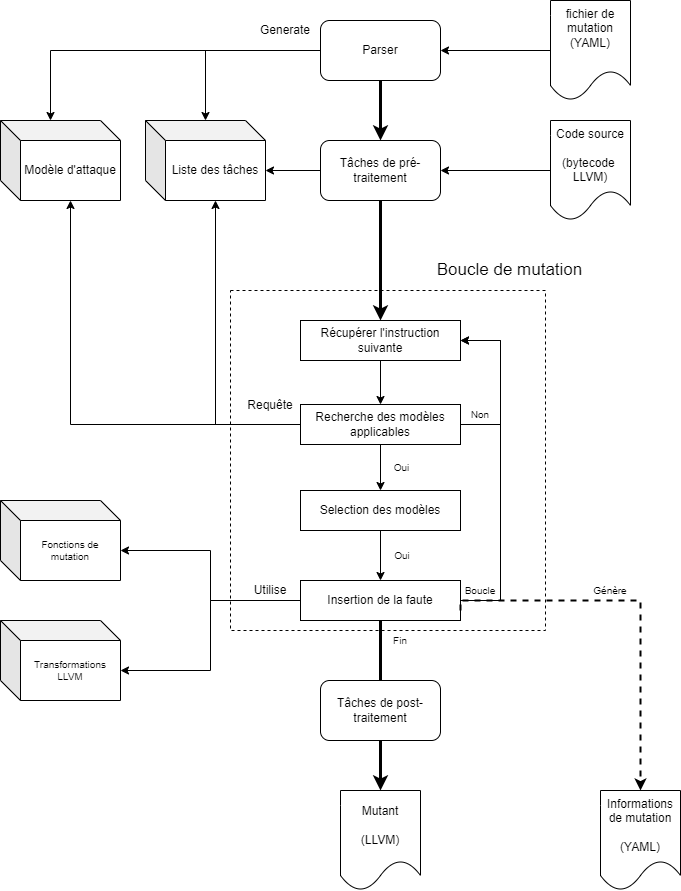
\includegraphics[scale=.52]{ch3-lazart/img/wolverine4-fr.drawio.png}
          \caption{Schéma général de \textit{Wolverine}  \label{fig:wolverine}}
        \end{figure}
        
        La figure \ref{fig:wolverine} présente le fonctionnement général d'une mutation.  
        Après la génération du modèle d'attaquant à partir du fichier de mutation (étape 1), l'étape de \textit{pré-traitement} (étape 2) consiste en plusieurs parcours du programme en fonction des opérations définies par l'utilisateur dans le fichier de mutation et l'instrumentation (détaillée en section \ref{sec:lazart-impl-preprocess}). 
        
        La \textit{boucle de mutation principale} parcourt chaque instruction du programme, fonction par fonction et bloc de base par bloc de base. Pour chaque instruction, le modèle d'attaquant et les informations des analyses sont interrogés afin d'obtenir la liste des modèles de faute applicables sur cette instruction. Le programme est transformé en fonction des modèles de faute sélectionnés. Ces transformations sont détaillées dans la section \ref{sec:lazart-impl-ip-transf}.
        Enfin, Wolverine génère le fichier \gls{llvm-ir} mutant qui sera transmis à KLEE. Il génère aussi certaines informations utilisées ensuite par Lazart, telles que la liste des points d'injection.
        
        \subsection{Fichier de mutation}
            \label{sec:lazart-impl-mutation-file}
            
            Le fichier de mutation contient les paramètres de la mutation sous la forme d'un fichier \gls{yaml} qui est soit fourni par l'utilisateur, soit généré depuis Lazart Core lorsque ceux-ci sont décrits directement en Python. Le listing \ref{lst:mutation-file-example-} montre un exemple de fichier de mutation.
                
\lstset{caption={Exemple de fichier de mutation},label=lst:mutation-file-example-}
\begin{lstlisting}  
---
# Example of mutation file for Wolverine
tasks: # Preprocessing tasks
  add_trace: 
    on: __mut__
  rename_bb: 
    on: __all__
  countermeasures:
    - on: __mut__
      type: load-duplication
## General fault models, can be reused on specific location by ID.
fault-models:
  - &data
    type: data
    all: 0 # All load are faulted to 0.
## Fault spaces. Uses fault models on specific location of the program.
fault-space:
  functions:
    __all__:
      models: [*data]
    foo:
      models: 
        - type: test-inversion
\end{lstlisting} 

            Le fichier de mutation contient trois parties: la section des tâches de pré-traitement (\texttt{tasks} ligne 3), la section des modèles de faute (\texttt{fault-models} ligne 12) et la section d'espace de faute (\texttt{fault-spaces} ligne 17). 
            La section des tâches contient un ensemble d'actions effectuées en pré-traitement ou post-traitement. Dans l'exemple \ref{lst:mutation-file-example-}, les tâches \texttt{add-traces} (l'ajout des \texttt{printf} de trace d'exécution), \texttt{rename-bb} (renommage des blocs de base) et \texttt{countermeasures} (application d'une contre-mesure, ici la duplication des \texttt{load}) sont définies. Le champ \texttt{on} définit l'ensemble des fonctions sur lesquelles la tâche est effectuée, \texttt{\_\_mut\_\_} et \texttt{\_\_all\_\_} étant des mots clefs prédéfinis correspondants respectivement à l'ensemble des fonctions sur lesquelles au moins un modèle est défini et l'ensemble de toutes les fonctions.
            
            La section de l'espace de faute suit une structure identique à celle du champ \texttt{attack\_model} (modèle d'attaquant) de l'\gls{api} Python (voir section \ref{sec:lazart-am-py}) et contient une association entre des points du programme (ici des fonctions) et des modèles de faute. Ces modèles peuvent être définis en-place ou par référence \gls{yaml} (comme ligne 20 dans l'exemple: \texttt{[*data]}).

        \subsection{Phase de pré-traitement}
        \label{sec:lazart-impl-preprocess}
        
            La phase de pré-traitement est effectuée au début de la passe de mutation. Celle-ci applique un ensemble d'opérations en fonction du fichier de mutation.
            
            Les opérations utilitaires (renommage de blocs de base), de trace (ajout de \texttt{printf} pour tracer les blocs de base pour l'étape de rejeu) ou encore d'ajout de contre-mesures automatiques sont appliquées lors de cette phase avec une granularité de l'ordre de la fonction ou du bloc de base. 
            Le pré-traitement effectue aussi les opérations déterminées par l'instrumentation du programme.            
            
            Cette phase pourrait aussi être utilisée pour appliquer d'autres analyses préliminaires (comme celles décrites dans la section \ref{lazart:metho}).
            Dans la première version de l'outil \cite{Potet/ICST14}, le modèle d'inversion de test était précédé par une phase de "coloration de graphe" effectuée dans un module externe en Java permettant de réduire l'espace de faute. 
            L'objectif d'attaque était alors défini en termes d'accessibilité à un bloc précis et cette analyse consiste à colorer chaque bloc pour savoir si une faute en inversion de test vers les branches then, else ou les deux peut mener au bloc ciblé.
            La combinaison de modèles de faute et la gestion de l'inter-procédural compliquent l'analyse dans les versions modernes de Lazart mais il s'agit aussi d'une analyse qui pourra être implémentée dans la phase de pré-traitement.
            
        \subsection{Boucle de mutation et points d'injection}
        \label{sec:lazart-impl-ip-transf}
        
            La boucle de mutation effectue une passe sur toutes les instructions du programme dans les fonctions spécifiées par le modèle de faute comme présenté dans la figure \ref{fig:wolverine}.
            Elle maintient en parallèle l'état des indications de l'instrumentation en fonction des primitives rencontrées dans le programme, telles que l'activation ou la désactivation de modèles (voir section \ref{sec:lazart-am-instr}).
            
\lstset{caption={Boucle de mutation de Wolverine},language=python, label=lst:wolv-mut-loop}
\begin{lstlisting}  
def mutation_loop(module: LLVMModule, istate: InstrumentationState, am: AttackModel):
    for function in llvm_module:
        istate.reset_function();
        for bb in basic_block:
            istate.reset_bb();
            for instr in bb:
                consumed = istate.handle(instr)
                if consumed:
                    continue
                    
                models = am.get_appliable_models(instr, istate)
                if len(models) > 0:
                    model = models[0]
                    if len(models) > 1: 
                        warning("several models appliable, selecting: " + model)
                    (instr, bb) = models.apply(instr)  
\end{lstlisting}

            Le listing \ref{lst:wolv-mut-loop} présente le pseudo-code de la boucle de mutation principale de Wolverine. Toutes les fonctions sont parcourues (à l'exception de primitives de \gls{llvm} et de Lazart) afin de pouvoir y détecter une activation de modèle par l'instrumentation\footnote{Le surcoût de performances est négligeable, toute l'étape de mutation étant elle-même négligeable.}.
            Comme le montre l'avertissement à la ligne de 15, Lazart considère que plusieurs modèles applicables sur une même instruction correspond à une erreur de configuration (par exemple si deux modèles de mutation de donnée s'appliquent sur une même variable). La section \ref{sec:wolverine-multi-ip} revient sur les cas où plusieurs fautes peuvent survenir sur un même point du programme.
            
            Une difficulté de la combinaison de modèles de faute est qu'il ne faut pas qu'un modèle s'applique sur du code qui est relatif à l'analyse (code de simulation des fautes, \texttt{printf} pour le rejeu etc.) et non au programme analysé.
            L'utilisation d'une seule passe permet de ne jamais muter deux fois une instruction (dès lors que les transformations sont locales) mais Wolverine utilise par ailleurs un système d'étiquettes sur les instructions lui permettant d'identifier quelles instructions sont relatives à un point d'injection, à une contre-mesure ou à l'affichage du rejeu par exemple.
            
            Wolverine fait le choix de limiter un maximum l'impact de la mutation sur le graphe de flot et le code original en englobant le code de déclenchement des points d'injection dans des \textit{fonctions de mutation} (section \ref{sec:lazart-impl-mfct}). 
            Ce choix permet aussi de simplifier le code muté s'il doit être utilisé par d'autres outils ou examiné manuellement, en permettant d'identifier simplement les parties du programme correspondant aux points d'injection.
            Cela étant, cette sur-couche d'un appel de fonction peut avoir des conséquences sur les performances de KLEE (discuté dans la section \ref{sec:lazart-mfct-inl}). 

            Le listing \ref{lst:llvm-mutable} contient un exemple de code \gls{llvm-ir} qui va permettre d'illustrer le fonctionnement de ces fonctions. Le listing \ref{lst:llvm-mutable-c} donne l'équivalent C de ce programme. 
            
            \begin{minipage}{0.93\linewidth}
            \begin{lstlisting}[style=base, caption={IR LLVM source}, label=lst:llvm-mutable]
µ%1 = load i32* %val, align 4µ            ; lecture de val
%2 = call i32 @foo(i32 %1)              ; appel de foo
%3 = icmp ne i32 %2, 0                  ; comparaison
§br i1 %4, label %else, label %then§      ; branchement conditionnel

\end{lstlisting}      
                
            \begin{lstlisting}[style=base, caption={Équivalent en langage C}, label=lst:llvm-mutable-c]
if(foo(val)) {
  // then:
} else {
  // else:
}
            \end{lstlisting} 
            \end{minipage}
            
            Dans cet exemple, pour un modèle de faute de mutation de donnée, la ligne 1 du programme est un point d'injection où la faute revient à charger une autre valeur que celle de \texttt{\%val}. De la même manière, une faute dans le modèle d'inversion de test peut être représentée par la négation de la condition de l'instruction \texttt{br} ligne 4. Ces deux points d'injection sont nommés respectivement $IP_{data}$ et $IP_{ti}$. 
         
            \begin{minipage}{0.93\linewidth}
            \begin{lstlisting}[style=base, caption={IR LLVM muté}, label=lst:llvm-mutated]
[...]
µ%6 = alloca i32
%7 = load i32* %val, align 4
%_LZ__w_call_ip_1 = call i32 @_LZ__mut_dl_i32(i32 %7, i8* getelementptr inbounds ([2 x i8], [2 x i8]* @_LZ__w_ip_1_id, i32 0, i32 0))
store i32 %_LZ__w_call_ip_1, i32* %6, align 4
%8 = load i32* %6, align 4µ
%9 = call i32 @foo(i32 %8)
%12 = icmp ne i32 %9, 0
§%_LZ__w_call_ip_2 = call i32 @_LZ__mut_ti(i32 %12, i8* getelementptr inbounds ([2 x i8], [2 x i8]* @_LZ__w_ip_1_id, i32 0, i32 0), i8* getelementptr inbounds ([5 x i8], [5 x i8]* @_LZ__w_ip_0_targetA, i32 0, i32 0), i8* getelementptr inbounds ([5 x i8], [5 x i8]* @_LZ__w_ip_0_targetB) 
br i1 %_LZ__w_call_ip_2, label %bb26, label %bb25§
            \end{lstlisting}
            \end{minipage}
            
            Le listing \ref{lst:llvm-mutated} présente la transformation du programme \ref{lst:llvm-mutable} à l'aide de fonctions de mutation pour les points d'injection $IP_{data}$ et $IP_{ti}$, respectivement représentés en rouge et en bleu-vert.
            Les fonctions de mutation (ici \texttt{\_LZ\_\_mut\_dl\_i32} et \texttt{\_LZ\_\_mut\_ti}) prennent en argument la valeur originale de l'opérande cible, une chaîne de caractère correspondant à l'identifiant (unique) du point d'injection et d'éventuels arguments supplémentaires nécessaires au modèle.
            L'opérande de l'instruction ciblée est passée à la fonction de mutation dont le retour est utilisé comme nouvelle opérande. 
            
            Dans le cas de la mutation de donnée, une variable temporaire est créée puisque la valeur non fautée $\%val$ doit être chargée avant d'être passée à la fonction de mutation, et l'instruction \texttt{load} ligne 6 nécessite une adresse (\texttt{i32*}) comme opérande. Cette valeur temporaire est ainsi créée avec l'instruction \textit{alloca} ligne 2, initialisée ligne 3, et finalement le retour de fonction \texttt{\%\_LZ\_\_w\_call\_ip\_1} est stocké dans la valeur temporaire avec une instruction \texttt{store} ligne 5, puis utilisé comme opérande pour l'instruction \texttt{load} ciblée par la faute ligne 6. Ainsi, il n'est pas nécessaire de modifier toutes les instructions du programme qui utilisent le temporaire \texttt{\%8} puisque celui-ci reste inchangé.

            Le modèle \gls{JMP} n'est pas géré nativement par Wolverine et la transformation de leurs points d'injection est effectuée à la compilation via l'instrumentation.
            Le modèle est cependant reconnu durant la boucle de mutation afin de supporter les points d'injection générés par l'utilisateur dans les analyses (l'\gls{api} Python ayant accès à ces points d'injections via le fichier \texttt{injection\_points.yaml}). 
                
    \section{Émulation des fautes}
    \label{sec:lazart-impl-mfct}
    
        Cette section s'intéresse à l'implémentation de l'émulation des fautes, que ce soit dans les fonctions de mutation ou dans les transformations de points d'injection.
        L'objectif de ces transformations est de retarder l'introduction des variables symboliques ainsi que les disjonctions de chemins et de couper au plus tôt l'exploration des chemins.
        
        La section \ref{sec:lazart-mfct-base} présente la structure des fonctions de mutation et propose une comparaison de plusieurs approches.
        La section \ref{sec:lazart-mfct-data} se concentre sur le modèle de mutation de données symboliques qui inclut une variable symbolique supplémentaire et discute des différentes versions de fonctions de mutation utilisées.
        La section \ref{sec:lazart-mfct-inl} discute des problématiques induites par les fonctions de mutation par rapport à une transformation en-place et des différentes solutions.
        La section \ref{sec:wolverine-multi-ip} parle de l'implémentation des points d'injection multiples générés par l'instrumentation.
 
        \subsection{Fonctionnement}
        \label{sec:lazart-mfct-base}
            
                Le programme présenté dans le listing \ref{lst:mfct-base} correspond au pseudo-code d'une émulation de faute sous la forme d'une fonction de mutation. 
                Les entrées sont la valeur originale \texttt{orig}, potentiellement symbolique, le compteur de fautes \texttt{fcount} (symbolique). La limite de fautes \texttt{flimit} est globale. 
                Les différents prédicats de chemins sont indiqués en marron et la mémoire symbolique (indiquée en rouge) considère \texttt{orig} comme concrète en entrée pour cet exemple.
                
             \begin{center}
            \lstset{basicstyle=\large}
            \lstset{language=C,style=codeC}    
            \begin{lstlisting}[caption=Pseudo-code de l'émulation des fautes, escapeinside={(*}{*)}, language=python, label=lst:mfct-base]
def mutation_fct(orig, fcount): (*{\color{brown} $PC_0 \equiv PC_{fcount}$ }*) (* {\color{red} $\sigma \: = \: \{ \: fcount \: \to \: fcount_0 \}$}*)
    if fcount >= flimit: # No sym variable. (*{\color{brown} $PC_1  \equiv PC_0 \land fcount \geq flimit $}*)
        return orig      
    (*{\color{brown} $PC_2 \: \equiv \: PC_0 \land fcount < \: flimit $}*)
        
    inject = sym_bool() # New sym variable.  (* {\color{red} $\sigma \: = \: \{ \: fcount \: \to \: fcount_0 \: \land \: inject = inject_0 \}$}*)
    if inject: (*{\color{brown} $PC_3  \equiv PC_2 \land inject = true $}*)
        fcount++ # Update. (* {\color{red} $\sigma \: = \: \{ \: fcount \: \to \: fcount_0 + 1\: \land \: inject = inject_0 \}$}*)
        if klee_is_replay(): # Do not create new paths.
            print(fault_str_with_params) # Trace fault trigger for replay.
        return faulted_value
    (*{\color{brown} $PC_4  \equiv PC_2 \land inject = false $}*)

    return orig
                \end{lstlisting}    
            \end{center}     

            Cette implémentation vise à retarder au maximum la création de la variable symbolique booléenne \texttt{inject}. C'est pourquoi un premier test sort immédiatement de la fonction si la limite de fautes est atteinte. C'est aussi la raison pour laquelle \textit{klee\_assume} n'est pas utilisée ici, son appel n'étant pas possible avant la création d'\texttt{inject}.
            La fonction \textit{klee\_is\_replay} est une primitive de KLEE permettant de ne pas exécuter le code lié au rejeu des traces durant l'exécution concolique, qui évite les risques de concrétisation \footnote{La documentation de KLEE indique que la fonction \texttt{printf} est gérée de façon spéciale, de manière à ne pas introduire de concrétisation. Mais nos expérimentations ont mit en évidence certains cas où la présence d'un appel à \texttt{printf} dépendant de variables symboliques fait manquer des chemins à KLEE.}.
 	
        \subsection{Mutation de données}
        \label{sec:lazart-mfct-data}
            
            Cette section vise à présenter les différentes approches d'émulation de fautes en données.
            Le listing \ref{lst:mut-data} présente le pseudo-code du retour de la valeur dans le cadre d'une faute des cinq approches d'implémentation de la fonction de mutation pour l'injection sur les données:
            \begin{itemize}
                \item \texttt{sym}, la variable symbolique injectée n'est pas contrainte et est retournée directement.
                \item \texttt{sym\_pred}, la fonction retourne un booléen déterminant si la valeur est valide, et qui est vérifié par un appel à \texttt{klee\_assume}. 
                \item \texttt{sym\_fun}, la valeur est transformée par la fonction qui retourne une nouvelle valeur contrainte.
                \item  \texttt{fun}, consiste à faire la même opération sans passer par une valeur symbolique.
                \item \texttt{fixed}: est utilisée pour l'injection d'une valeur constante.
            \end{itemize} 
                
\lstset{language=python, caption={Différentes versions de contraintes la mutation de donnée},language=python,label=lst:mut-data}
\begin{lstlisting}   
# Symbolic raw (sym)
return sym_int()
    
# Symbolic constrained (sym_pred)
value = sym_int()
klee_assume(pred(value, original))
return value;

# Symbolic constrained (sym_fun)
value = sym_int()
return f(value, original)
    
# Not symbolic, apply function (fun)
return f(original)
    
# Fixed value (fix)
return N
                \end{lstlisting}

            
  
        \subsection{Performance et inlining}
        \label{sec:lazart-mfct-inl}
 	
 	        Cette section compare les approches par fonction de mutation et par transformation en-place (c'est-à-dire sans appel de fonction, en transformant le graphe de flot local).
 	        Les fonctions de mutation ont l'avantage d'être plus simples pour un utilisateur qui souhaiterait créer de nouveaux modèles et parce qu'elles simplifient le code à analyser en séparant clairement le graphe de flot original de la partie mutation.
 	        Cependant, ces fonctions induisent une surcharge pour le moteur d'exécution symbolique, qui doit effectuer le changement de contexte dû à un appel de fonction et transmettre des paramètres statiques en argument (comme la chaîne de caractères correspondant à l'identifiant de point d'injection, ou l'entier \texttt{fcount} correspondant au nombre de fautes injectées par exemple), et les auteurs de REFINE \cite{Georgakoudis/ICHPCNSA17} indiquent que l'implémentation en-place permet d'obtenir des meilleures performances.
 	        Néanmoins, les expérimentations menées pour Lazart monstrent que ce surcoût n'est pas si important dans le cas d'une exécution concolique avec KLEE, l'explosion des chemins due aux fautes ayant un impact bien plus important que cette surcharge sur certains exemples.
 	        
            Wolverine propose une option d'inlining automatique des fonctions de mutation via une passe \gls{llvm} qui est par défaut appliquée sur chaque appel de fonction de mutation (généré ou défini par l'utilisateur). Cette approche n'effectue pas un inlining en-place, mais place le code de la fonction de mutation dans la fonction courante (qui est donc réutilisé par d'autres injections dans la même fonction). Cette approche souffre de la surcharge de la transmission des arguments tout comme la version avec fonction de mutation, mais ne contient pas d'appel de fonction explicitement (instruction \texttt{call}).
            Une version en-place de la mutation de donnée symbolique a aussi été implémentée, qui elle consiste à avoir un code de mutation séparé pour chaque point d'injection.
            
            La table \ref{tbl:inlining} compare l'approche des fonctions de mutation sans optimisation (\texttt{mfct}), l'inlining automatique (\texttt{mfct+inl}) et la mutation en-place (\texttt{inplace}) sur un ensemble de programmes. Les exemples utilisés sont indiqués dans la colonne "Prgm.", $rsa0$ correspondant à l'implémentation de \gls{rsa} en mise-à-0 et $loader$ au bootloader (voir chapitre précédent). $loader$ n'est évalué qu'en faute unique.
            L'approche utilisée est indiquée dans la colonne "Stratégie", la version en-place n'étant pas implémentée pour l'injection d'une valeur fixe, la version en-place pour $rsa0$ n'est pas présente.
            Les colonnes suivantes indiquent le nombre d'attaques trouvées en fonction du nombre de fautes. On constate que chaque version donne bien des résultats identiques. 
            
            Les colonnes "Chemins" et "Instrs." indiquent respectivement le nombre de chemins explorés et le nombre d'instruction exécutées. On constate que l'inlining automatique est moins performant.
            La colonne "TDSE" qui indique le facteur de temps d'exécution moyen indexé sur l'approche la plus faible. Les variations entre les versions \texttt{mfct} et \texttt{mfct+inl} sont trop faibles pour être mesurées dans le cas de $rsa0$ mais visibles sur $loader$. 
            Le fait que l'inlining automatique soit plus coûteux tend à montrer que les changements de contexte lié à l'appel de fonction sont négligeables pour KLEE. La différence entre les deux étant expliquée par le fait que l'inlining automatique de \gls{llvm} complexifie légèrement le graphe de flot.
            En revanche, l'exemple $loader$ indique des facteurs de temps plus significatifs. La version \texttt{inplace} étant la plus performante puisque les passages d'arguments ne sont pas présents.
            
            Les colonnes "ICov" et "BCov" donnent des indications concernant la couverture des instructions et des blocs de base. La différence entre les approches est significative mais principalement parce que ces métriques ne mesurent pas la même chose suivant les versions.
            Dans le cadre d'une approche \texttt{mfct}, chaque point d'injection partage son code avec tous les points d'injection utilisant la même fonction de mutation. La couverture donnée par KLEE reflète donc davantage celle obtenue sur le programme analysé.
            Dans le cadre de l'inlining automatique \texttt{mfct+inl}, la couverture du code d'émulation est liée à la fois à la fonction de mutation utilisée, mais aussi à la fonction contenant le point d'injection.
            Pour la mutation en-place, le code d'émulation est séparé pour chaque point d'injection et la couverture retournée par KLEE est donc plus faible.
            On constate d'ailleurs que le nombre de chemins explorés est le même pour toutes les approches, seul le nombre d'instructions exécutées diffère.
            
            \begin{table}[ht]
            \centering
            \small
            \setlength\tabcolsep{4pt} % default value: 6pt
            \begin{tabular}{l|l|llll|lll|lll}
            Prgm. & Stratégie & 1F & 2F & 3F & 4F & Ktests & Chemins & Instrs. & ICov & BCov & TDSE \\
            \hline
            \hline
            rsa0 & mfct & 10 & 33 & 65 & 92  & 202 & 913 & 52965525 & 100 & 100 & \textbf{1} \\
            & mfct+inl & 10 & 33 & 65 & 92 & 202 & 913 & 52969338 & 98.55 & 93.02 & \textbf{1} \\
            \hline
            loader & mfct & 12 & - & - & - & 14 & 13592 & 218071560 & 59.7 & 45.26 & 1.15 \\
            & mfct+inl & 12 & - & - & - & 14 & 13592 & 237171222 & 69.65 & 58.39 & 1.3 \\
            & inplace & 12 & - & - & - & 14 & 13592 & 183262082 & 64.06 & 58.39 & \textbf{1}
            \end{tabular}
            \caption{Expérimentations sur la mutation de données}
            \label{tbl:inlining}
            \end{table}
                
            La table \ref{tbl:inlining-resume} présente une comparaison des approches d'émulation des fautes.
            La colonne "Performance" classe les approches en fonction de la surcharge du temps d'exécution.
            La seconde colonne s'intéresse à l'impact de la méthode sur les métriques de couverture de KLEE.  
            Les colonnes suivantes indiquent respectivement la simplicité avec laquelle un modèle peut être ajouté ou étendu (l'implémentation au niveau source étant considérée plus simple que la manipulation de la représentation \gls{llvm}), et si le code d'émulation est explicitement séparé du reste du programme.
            La dernière colonne indique l'état de l'implémentation de la méthode dans Lazart. La version en-place n'est disponible que pour la mutation de donnée non-contrainte\footnote{Hors Wolverine, le modèle \gls{JMP} est un exemple d'émulation en-place.}. Une version en-place pour les autres modèles de Lazart est une piste d'amélioration de l'outil.
            
            \begin{table}[ht]
            \centering
            \small
                \setlength\tabcolsep{3pt} 
                \begin{tabular}{l|l|l|l|l|l}
                Approche & Performance & \begin{tabular}[c]{@{}l@{}}Représentativité\\ de la couverture\end{tabular} & \begin{tabular}[c]{@{}l@{}}Extensibilité des\\ modèles\end{tabular} & \begin{tabular}[c]{@{}l@{}}Séparation \\ de l'émulation\end{tabular} & Implémenté \\
                \hline
                \hline
                mfct & moyenne & par modèle & simple & forte & oui (défaut) \\
                \hline
                mfct+inl & pire & \begin{tabular}[c]{@{}l@{}}par modèle et\\ par fonction\end{tabular} & simple & moyenne & oui \\
                \hline
                inplace & meilleure & par IP & complexe & aucune & partielle (dl-sym)
                \end{tabular}
            \caption{Comparaison des approches de mutation de point d'injection}
            \label{tbl:inlining-resume}
            \end{table}
                
            \subsection{Points d'injection multiples}
            \label{sec:wolverine-multi-ip}
            
                Un point d'injection multiple consiste à faire une disjonction entre le cas nominal et plusieurs cas fautés, comme indiqué dans le listing \ref{lst:multi-ip}. 
                Les points d'injection multiples sont plus performants qu'une succession de points d'injection simples, puisqu'ils n'introduisent qu'une seule fois le chemin correspondant à l'absence de faute.
                Wolverine ne génère pas de point d'injection multiple pour l'inversion de test et la mutation de données puisque ceux-ci n'entrent pas en collision lors de leur application (voir section \ref{sec:lazart-impl-ip-transf}). Il serait cependant possible de créer des points d'injection multiples si d'autres modèles étaient ajoutés.
                Le modèle \gls{JMP} (uniquement défini par instrumentation) est un exemple de point d'injection multiple dans Lazart, lorsque plusieurs étiquettes de destination sont spécifiées. 
                
                \begin{minipage}{0.93\linewidth}
\lstset{caption={Pseudo-code d'un point d'injection multiple},label=lst:multi-ip}
\begin{lstlisting}    
int select = sym_int()
if select == 0:
  normal_behavior()
else if select == 1:
  model_1_behavior()
else if select == 2:
  model_2_behavior()
...                \end{lstlisting}    
                \end{minipage}         

                La table \ref{tbl:multi-ip} présente les résultats normalisés (sur la valeur la plus faible indiquée en gras) sur un ensemble de programmes \texttt{verify\_pin} ($vp0$ à $vp6$) avec deux modèles de fautes \gls{JMP} : le saut vers deux étiquettes possibles et le saut vers trois étiquettes possibles.
                La colonne "Mode" indique si le point d'injection est émulé par une succession de points d'injection simples ("unique") ou bien par un point d'injection multiple ("multiple"). 
                On peut constater que la version avec \gls{ip}s multiples est plus performante en explorant moins de chemins, sans différence sur les résultats de l'analyse d'attaque obtenus.
                
            \begin{table}[h]
            \centering
\begin{tabular}{l||l|l|l|l}
Mode & TDSE & Traces & Chemins explorés (EP) & Attaques \\
\hline
\hline
unique & 1.43 & 1.25 & 1.80 & \textbf{1} \\
\hline
multiple & \textbf{1} & \textbf{1} & \textbf{1} & \textbf{1}
\end{tabular}
            \caption{Métriques de performance entre IP simple et multiple}
            \label{tbl:multi-ip}
\end{table}
        
 	\section{Implémentation des traitements}
 	\label{sec:lazart-impl-analysis}
 	
 	    Cette section se focalise sur l'implémentation et la complexité des traitements proposés par Lazart (présentés en section \ref{sec:lazart-formal}).
 	    La section \ref{sec:lazart-impl-analysis-linear} se concentre sur les analyses d'attaques et de points chauds, et 
 	    la section \ref{sec:lazart-impl-analysis-aar} sur l'analyse de redondance-équivalence.
 	
 		\subsection{Attaques et points chauds}
 		\label{sec:lazart-impl-analysis-linear}
 		
 		    L'analyse d'attaque et l'analyse de points chauds sont des analyses linéaires puisqu'elles ne s'appliquent qu'une fois sur chaque trace. Leur complexité au pire cas est donc $O(n * m)$, avec $n$ le nombre de traces à parcourir et $m$ la taille moyenne des traces (en nombre d'évènements à analyser).
 		    L'analyse de points chauds est cependant plus coûteuse en temps parce qu'elle maintient plusieurs valeurs pour chaque point d'injection.  
 		    
            \begin{figure}[H]\centering
            \begin{multicols}{2}
\lstset{language=python, caption={Pseudo-code de l'analyse d'attaque},label=lst:aa-code, showlines=true}
\begin{lstlisting}
def attack_analysis(a: Analysis, s_fct):
    attacks = []
    for order in range(a.max_order()):
        for trace in traces_list(a, order, s_fct):
            attacks.append(trace)
    return attacks






\end{lstlisting}  
\columnbreak

\lstset{language=python, caption={Pseudo-code de l'analyse de points chauds},label=lst:hsa-code}
\begin{lstlisting}
def hotspots_analysis(a: Analysis, s_fct):
    ips_data = dict<ip_id: str, data: IPData>
    
    for order in range(a.max_order()):
        for trace in traces_list(a, order, s_fct):
            data = compute_local_hs(trace) # metrics on ip in the traces
            ips_data.update(data) # update metrics
    
    return ips_data
\end{lstlisting}  
\end{multicols}
            \caption{Pseudo-code pour les analyses d'attaques et de points chauds}
            \label{fig:implem-aa-hs}
            \end{figure}
            
            Le listing \ref{lst:aa-code} (de la figure \ref{fig:implem-aa-hs}) correspond au pseudo-code de l'analyse d'attaque, qui peut se réduire à un filtrage des traces suivant le prédicat \texttt{s\_fct} fourni par l'utilisateur (par défaut les traces satisfaisant l'objectif d'attaque, sans terminaison en erreur).
            
            Le listing \ref{lst:hsa-code} présente le pseudo-code du calcul des points chauds qui correspond à une mise-à-jour des valeurs (nombre total de déclenchements, nombre maximum par trace etc...) pour chaque trace, l'ensemble de traces étant aussi paramétré par \texttt{s\_fct}.
 		    
            Les deux analyses pourraient en théorie être effectuées toutes deux en une seule passe mais la séparation permet d'appliquer l'analyse de points chauds sur d'autres ensembles de traces (comme les attaques minimales par exemple).
 		    
        \subsection{Analyse de redondance-équivalence}
        \label{sec:lazart-impl-analysis-aar}
            
            L'analyse de redondance-équivalence a une complexité plus élevée que les analyses d'attaques et de points chauds.
            Le temps d'analyse peut avoir un impact non négligeable sur les performances pour certains exemples, comme cela a été illustré dans la section \ref{sec:lz:exp:results}.
            
            L'analyse d'équivalence nécessite de comparer pour chaque ordre $o$ (chaque nombre de fautes) toutes les traces du groupe de traces entre elles, ce qui implique une complexité au pire cas pour un ordre donné en $O(n * n * m)$, avec $n$ le nombre de traces pour un ordre donné et $m$ la moyenne de la taille des traces dans cet ensemble. 
            Plus il existe de classes d'équivalence, plus l'analyse est rapide (pour chaque groupe d'équivalence, une seule trace est traitée par l'analyse de redondance). La complexité à l'ordre $o$ serait plutôt $O(n * e * m)$ avec $e$ correspondant au nombre de classes d'équivalence pour $o$. 
            
            L'analyse de redondance nécessite de comparer chaque trace d'ordre $o$ à toutes les traces de chaque ordre supérieur.
            La complexité correspond donc à $O(n * log(n))$.
            Si on ne s'intéresse qu'à trouver les attaques minimales (voir section \ref{sec:lazart-redundancy}), il n'est pas nécessaire de calculer toutes les relations de redondance entre les traces, et les traces déjà déterminées comme redondantes n'ont pas à être comparées aux autres traces.
            L'option \texttt{lazy} permet de limiter l'analyse de redondance à la recherche de traces minimales. 
       
            Le listing \ref{lst:red-min-code} présente le pseudo-code de l'analyse de redondance-équivalence.
            Le graphe de redondance (\texttt{graph}) représente les relations de redondance entre les traces ainsi que les classes d'équivalence.
            Les classes d'équivalence sont d'abord calculées pour chaque nombre de fautes et l'analyse de redondance peut ainsi s'appliquer au niveau de ces classes plutôt que sur chaque trace.
            Les métriques, comme le nombre total d'attaques minimales, de classes d'équivalence minimales ne sont pas présentées ici mais sont calculées et stockées durant l'analyse (afin de ne pas avoir à retraverser le graphe de redondance pour récupérer ces valeurs).
            
    \lstset{language=python, caption={Pseudo-code de l'analyse de points chauds},label=lst:red-min-code}
    \begin{lstlisting}
    def equivalence_then_redundancy(a: Analysis, do_eq: bool, do_red: bool, eq_s_fct, red_s_fct, lazy: bool):
    graph = TraceGraph()
    
    if do_eq:
        for order in range(a.max_order()):
            trs = traces_list(a, order, eq_s_fct):
            for i in range(trs.size() - 1):
                tr1 = trs[i]
                for j in range(i, trs.size()):
                    tr2 = trs[j]
                    if equivalence_rule(tr1, tr2):
                        graph.set_equivalent(tr1, tr2)
                        
    for order in range(1, a.max_order() - 1): 
        trs = traces_list(a, order, red_s_fct)
        for tr1 in trs:
            if graph.redundant(tr1) and lazy: # lazy mode 
                continue
                
            for target_order in range(order + 1, a.max_order()):
                for tr2 in traces_list(a, order, red_s_fct):
                    if redundancy_rule(tr1, tr2):
                        graph.set_redundant(tr1, tr2)
                
    return graph
    \end{lstlisting}   
            
            Cette approche, consistant à réduire la complexité de la redondance en calculant préalablement les classes d'équivalence, est efficace si peu de classes d'équivalence sont créées.
            Il est possible à l'inverse de commencer par calculer la redondance des traces puis ne calculer l'équivalence que sur les attaques minimales.
            Si le nombre de classes d'équivalence est élevé pour les attaques maximales et centrales, alors cela peut accélérer le calcul de l'équivalence. 
            
            L'implémentation de Lazart permet de paramétrer l'ordre dans lequel l'équivalence et la redondance sont effectuées ainsi que les définition d'équivalence et de redondance utilisées. 
            L'utilisateur peut spécifier les prédicats déterminant l'équivalence et la redondance de deux traces, les plages d'ordres sur lesquelles les analyses s'appliquent, et les plages d'ordres de comparaison (voir la liste des options dans l'annexe \ref{annexe:lz:analysis-args}).
            
    \section{Conclusion et perspectives}
    \label{sec:lazart-conclusion}
    
        \subsection{Contributions sur Lazart}
        
            La reprise et le développement de l'outil Lazart ont été réalisés tout au long de cette thèse. 
            L'outil a été réécrit pratiquement en entier afin de répondre aux besoins des différents utilisateurs académiques et industriels. L'\gls{api} Python a été développée pour simplifier la création d'analyses complexes et Wolverine (phase de mutation) a été entièrement réécrit de manière à supporter la mutation inter-procédurale et la combinaison de modèles de fautes, ainsi que faciliter la récupération d'informations sur la mutation (comme les détails sur les points d'injection dans le mutant final). Le projet a part ailleurs été migré vers une version plus récente de \gls{llvm} (version 9) et de KLEE (version 2). 
            
            L'analyse de redondance a été revue au cours de la thèse puisque dans sa version originale \cite{Potet/ICST14} celle-ci n'utilisait qu'une version partielle de la définition sous-mot. Les concepts d'équivalence, de faute-équivalence et de redondance ont été implémentés, ainsi que l'analyse de points chauds et les analyses de contre-mesures présentées dans les chapitres suivants.
            
            L'analyse inter-procédurale et la combinaison de modèles de fautes ont été ajoutées, ainsi que les fonctionnalités de mutation par instrumentation du programme.
            Le projet compte environ 20k lignes de codes réparties entre les différents modules (\gls{api} Python, Wolverine et outils utilitaires). 
            De plus, la collection \gls{fissc} a été mise à jour au fur et à mesure du développement de Lazart. 
        
        \subsection{Pistes d'amélioration}
        \label{sec:future-work}
        
            Outres des améliorations techniques, certaines pistes sont envisagées pour le futur de Lazart. Les modèles de fautes supportés par l'outil pourraient être étendus. 
            En effet, les modèles \gls{JMP}, \gls{TI} et \gls{DL} permettent de simuler la plupart des modèles haut-niveaux. 
            Par exemple, il est possible de représenter \textit{test-falltrought} (exécuter les deux branches d'un test) à l'aide du modèle \gls{JMP}. 
            Le modèle de mutation de pointeurs pourrait aussi être simulé\footnote{Si on exclut la solution qui serait de rendre symbolique les adresses, non supportée par KLEE.} en autorisant l'injection d'une valeur contenue dans une variable locale de la même fonction ou bien encore en actualisant la mauvaise variable (ou la mauvaise adresse) lors de l'injection. 
            Des travaux sont en cours dans cette direction.
            
            \paragraph{}
            Les fautes permanentes ne sont pas traitées par Lazart, et pourraient être représentées avec l'utilisation de fonctions de mutation spécifiques par point d'injection (ou une mutation en-place). Le point d'injection serait ainsi activé définitivement une fois déclenché et la valeur retourné serait toujours retournée.
            Le support des fautes permanentes, en mémoire, ainsi que des limites de fautes spécifiques à un modèle de faute ou un point d'injection particulier (voir section \ref{sec:lazart:metho:static}) sont aussi des perspectives d'extension pour l'outil.
            
            
            \paragraph{}
            L'implémentation d'une version inter-procédurale de la coloration de graphe \cite{Potet/ICST14} pour le modèle d'inversion de test (ou plus généralement des modèles orientés flot de contrôle) afin d'écarter les fautes sur des points du programme n'ayant pas d'accessibilité avec l'objectif d'attaque pourrait améliorer les performances de ces modèles.
            Cela s'avère cependant plus complexe à mettre en place dans le cadre de la combinaison de modèles si les fautes peuvent ajouter des arrêtes ou des blocs. 
            Plus généralement, la mises en place d'analyses préliminaires pour Lazart (voir sections \ref{lazart:metho} et \ref{sec:lazart-impl-preprocess}) fait partie des projets futurs pour l'outil.
            
            \paragraph{}
            Plutôt que l'approche de type \textit{swifi} de Lazart qui consiste à émuler les fautes en mutant le programme avant de le transmettre à l'outil d'exécution symbolique, il est possible de modéliser les fautes dans le moteur d'exécution symbolique. En fonction d'un modèle d'attaquant, le moteur d'exécution peut diviser l'exécution symbolique en un comportement fauté et non fauté lorsqu'il rencontre une instruction sur laquelle une faute peut être injectée (voir l'exploration symbolique fautée décrite dans la section \ref{sec:dse-fi}). Dans le cas de \gls{llvm-ir}, cela rendrait notamment la simulation des fautes qui impliquent une modification du \gls{cfg} (ajout de blocs de base et ou d'arêtes) plus simple à simuler puisque cela reviendrait à modifier l'instruction suivante à lire pour le moteur d'exécution concolique, sans nécessiter une reconstruction d'un \gls{cfg} incluant tous les sauts possibles comme c'est le cas actuellement. 
            Les modèles de faute touchant spécifiquement des parties de la modélisation du système seraient aussi plus faciles à simuler.
            Par exemple, un modèle d'injection de données dans la mémoire\footnote{Dans Lazart ce type de faute peut être simulée avec une succession d'injections de mutation de donnée (fautes multiples en lecture). Une autre solution serait de développer un modèle d'injection de données sur l'instruction \texttt{store}.} reviendrait à rendre symbolique une portion de mémoire touchée.
            Bien entendu, la problématique d'explosion combinatoire en fautes multiples reste présente.
            
            L'implémentation dans le moteur d'exécution symbolique est probablement plus efficace en termes de performance en raison de l'économie des lectures / écritures de fichiers (voir section \ref{sec:lazart-impl-klee}) et des changements de contexte dûs à l'appel externe de l'outil concolique.
            Les analyses sur l'accessibilité ou la dépendance des données pourraient être faites au fur et à mesure de l'exécution symbolique. En effet, si une faute a déjà été injectée et qu'une limite de fautes est fixée, alors certains chemins fautés peuvent devenir impossibles en raison de cette limite (pareillement pour des analyses de teinte ou de dépendance).  
            De plus, l'accès à la représentation du système (représentation de la mémoire, système de fichiers, temporaires etc...) de l'outil d'exécution permettrait d'implémenter plus simplement des extensions de cette représentation pour certains modèles spécifiques (par exemple un registre multiplieur spécifique à une architecture \cite{Laurent/DATE19}).
            Des outils de ce type existent au niveau binaire mais aucun au niveau \gls{llvm-ir}.
            Une version étendue de KLEE supportant l'injection de fautes est donc une piste de recherche intéressante.
            
            \paragraph{}
            Une autre piste d'amélioration à explorer consiste à ne pas encoder l'objectif d'attaque dans le programme analysé à l'aide de \texttt{klee\_assume}, mais de le vérifier avec le prédicat de chemin.
            Cela permettrait d'éviter la problématique d'une exécution concolique non disjointe (voir section \ref{sec:eq}) à cause de cette vérification, les contraintes sur les entrées et l'objectif d'attaque étant simplement des contraintes supplémentaires au prédicat de chemin. Ne pas explorer les chemins dans le code d'encodage de l'objectif d'attaque permettrait d'améliorer le passage à l'échelle pour certaines analyses.